\documentclass{article}%
\usepackage[T1]{fontenc}%
\usepackage[utf8]{inputenc}%
\usepackage{lmodern}%
\usepackage{textcomp}%
\usepackage{lastpage}%
\usepackage{geometry}%
\geometry{margin=0.5in}%
\usepackage{graphicx}%
%
\title{Report on PlacementData dataset}%
\author{Auto2Class}%
\usepackage{amsmath}%
\usepackage{amssymb}%
\usepackage{enumitem}%
%
\begin{document}%
\normalsize%
\maketitle%
\newpage%
\tableofcontents%
\newpage%
\section{Exploratory Data Analysis}%
\label{sec:ExploratoryDataAnalysis}%
\subsection{Non{-}Null Count, Dtype of features}%
\label{subsec:Non{-}NullCount,Dtypeoffeatures}%


\begin{table}[h!]%
\caption{Dataset Columns Information}%
\vspace{0.2cm}%
\centering%
\begin{tabular}{|c||c||c||c|}%
\hline%
Index&Column&Non{-}Null Count&Dtype\\%
\hline%
0&sl\_no&215&int64\\%
1&gender&215&object\\%
2&ssc\_p&215&float64\\%
3&ssc\_b&215&object\\%
4&hsc\_p&215&float64\\%
5&hsc\_b&215&object\\%
6&hsc\_s&215&object\\%
7&degree\_p&215&float64\\%
8&degree\_t&215&object\\%
9&workex&215&object\\%
10&etest\_p&215&float64\\%
11&specialisation&215&object\\%
12&mba\_p&215&float64\\%
13&status&215&object\\%
14&salary&148&float64\\%
\hline%
\end{tabular}%
\end{table}

%
\subsection{Descriptive Statistics}%
\label{subsec:DescriptiveStatistics}%


\begin{table}[h!]%
\caption{Dataset Descriptive Statistics}%
\vspace{0.2cm}%
\centering%
\begin{tabular}{|c||c||c||c||c||c||c||c||c||c|}%
\hline%
Index&Column Name/Statistic&count&mean&std&min&25\%&50\%&75\%&max\\%
\hline%
0&sl\_no&215.0&108.0&62.21&1.0&54.5&108.0&161.5&215.0\\%
1&ssc\_p&215.0&67.3&10.83&40.89&60.6&67.0&75.7&89.4\\%
2&hsc\_p&215.0&66.33&10.9&37.0&60.9&65.0&73.0&97.7\\%
3&degree\_p&215.0&66.37&7.36&50.0&61.0&66.0&72.0&91.0\\%
4&etest\_p&215.0&72.1&13.28&50.0&60.0&71.0&83.5&98.0\\%
5&mba\_p&215.0&62.28&5.83&51.21&57.95&62.0&66.25&77.89\\%
6&salary&148.0&288655.41&93457.45&200000.0&240000.0&265000.0&300000.0&940000.0\\%
\hline%
\end{tabular}%
\end{table}

%
\newpage%
\subsection{Distribution of features}%
\label{subsec:Distributionoffeatures}%
\subsubsection{Histograms of Numerical columns}%
\label{ssubsec:HistogramsofNumericalcolumns}%


\begin{figure}[h!]%
\centering%
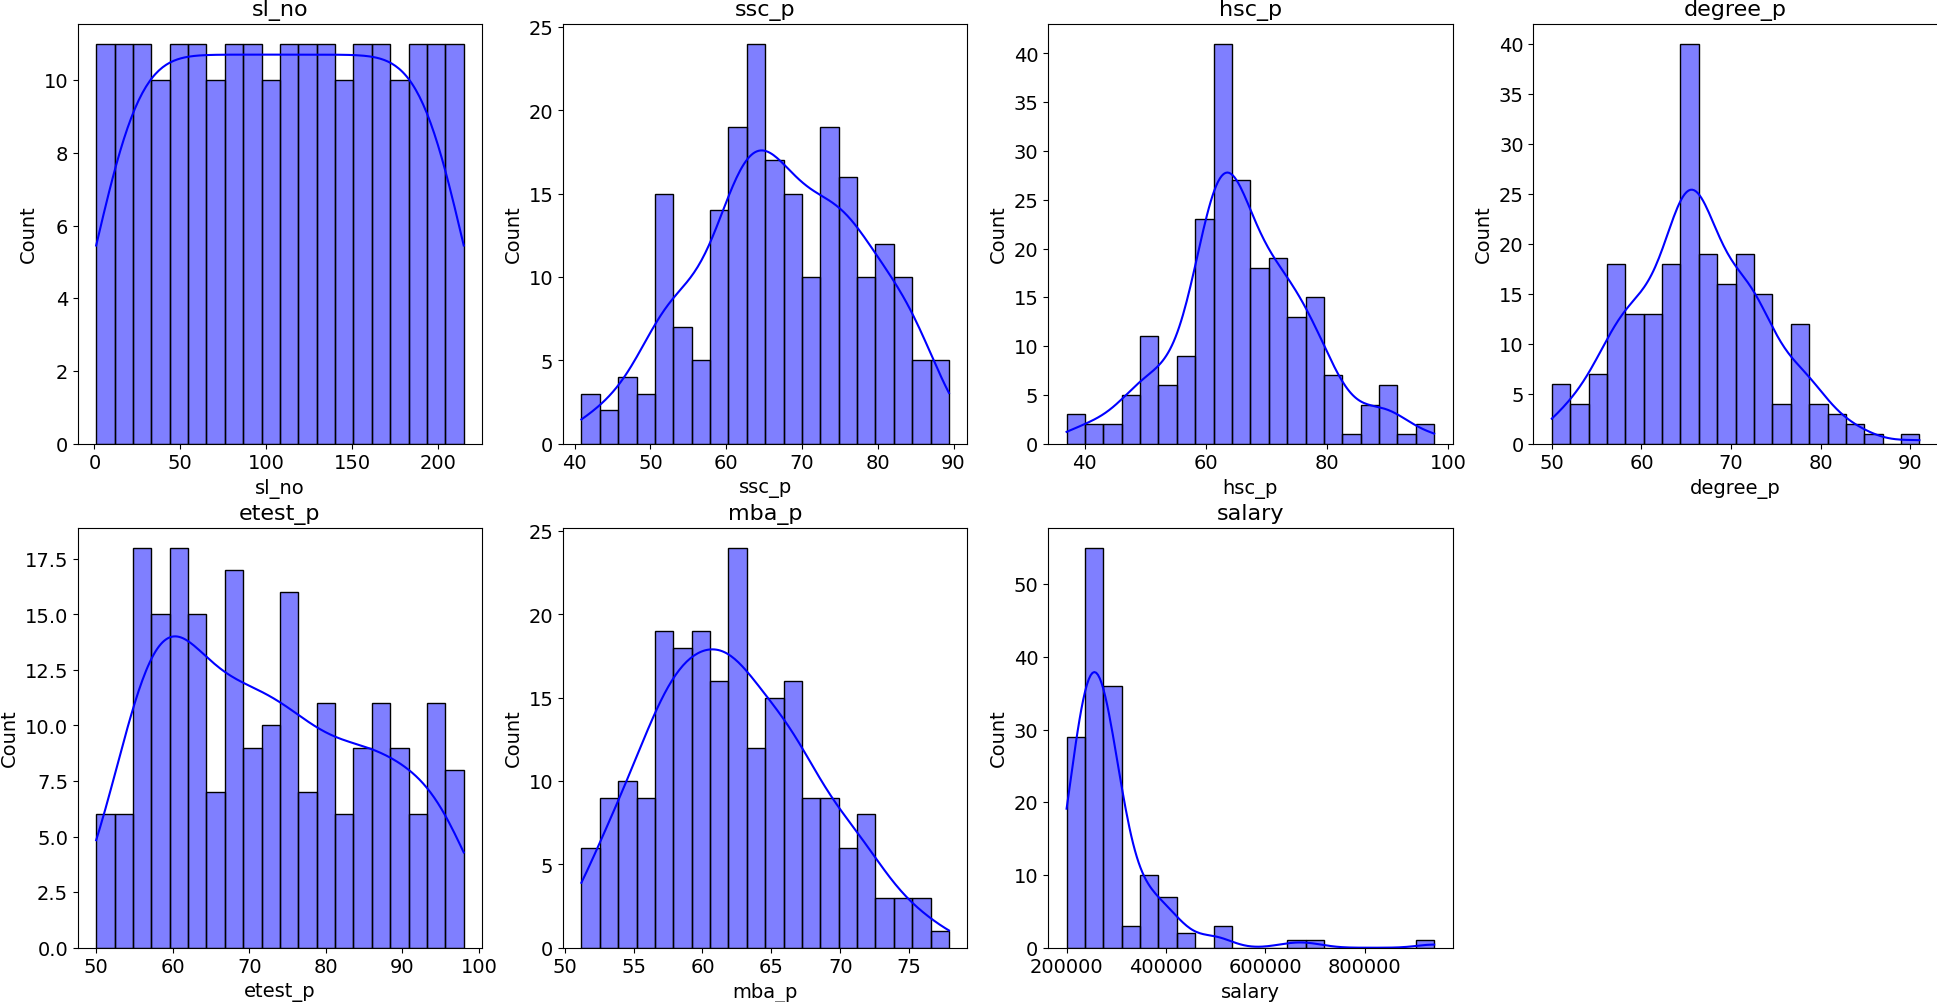
\includegraphics[width=460px]{EDA/histograms.png}%
\caption{Histograms of Numerical columns}%
\end{figure}

%
\newpage%
\subsubsection{Bar Charts of Categorical columns}%
\label{ssubsec:BarChartsofCategoricalcolumns}%


\begin{figure}[h!]%
\centering%
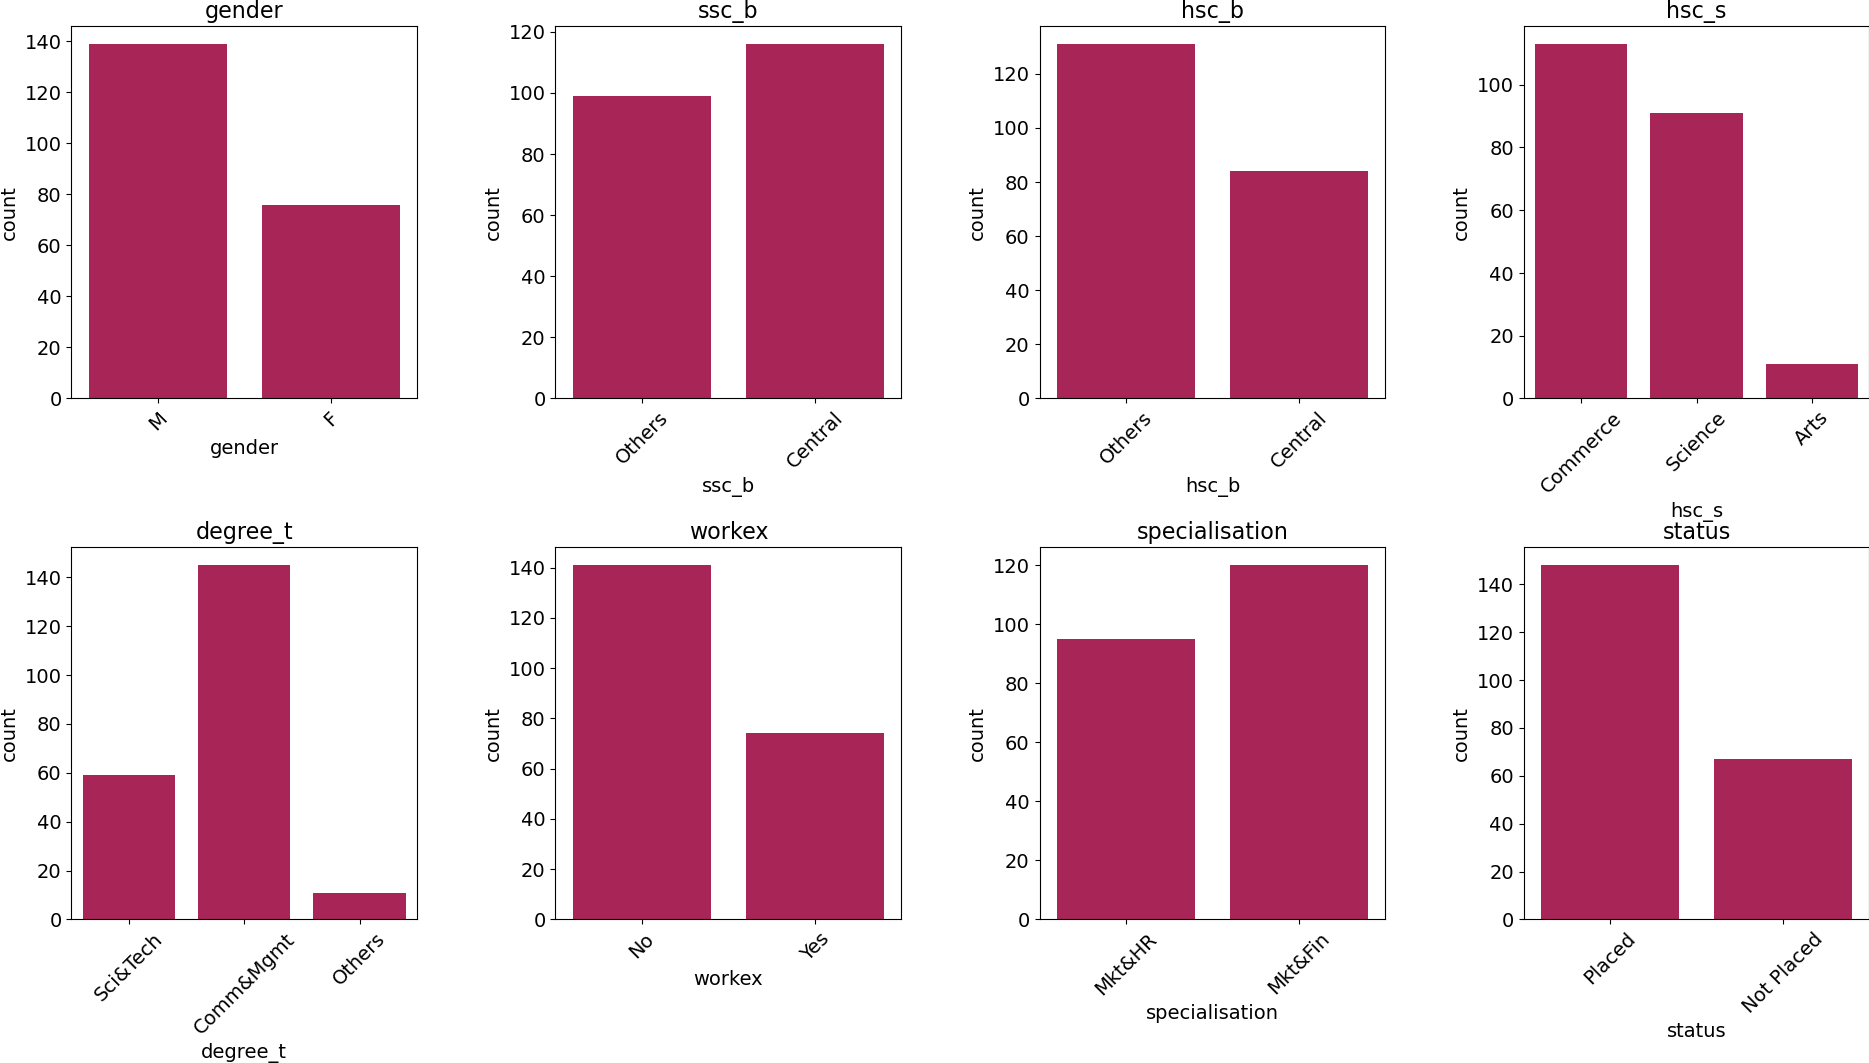
\includegraphics[width=460px]{EDA/bar_charts.png}%
\caption{Bar Charts of Categorical columns}%
\end{figure}

%
\newpage%
\section{Evaluation Metrics}%
\label{sec:EvaluationMetrics}%
\subsection{Accuracy}%
\label{subsec:Accuracy}%

                \textbf{Accuracy} is one of the simplest evaluation metrics for classification models. 
                It is defined as the ratio of correctly predicted observations to the total number of observations:

                \[
                \text{Accuracy} = \frac{\text{Number of Correct Predictions}}{\text{Total Number of Predictions}}
                \]

                While accuracy is intuitive and easy to understand, it may not be suitable for imbalanced datasets. 
                For example, in a dataset where 95\% of the samples belong to one class, predicting the majority class for every instance 
                would result in high accuracy but poor performance on the minority class.
                

%
\subsection{F1 Score}%
\label{subsec:F1Score}%

                The \textbf{F1 Score} is the harmonic mean of Precision and Recall, providing a balance between the two. 
                It is particularly useful when dealing with imbalanced datasets. Precision and Recall are defined as follows:

                \[
                \text{Precision} = \frac{\text{True Positives}}{\text{True Positives} + \text{False Positives}}
                \]
                \[
                \text{Recall} = \frac{\text{True Positives}}{\text{True Positives} + \text{False Negatives}}
                \]

                The F1 Score combines these metrics:

                \[
                \text{F1 Score} = 2 \cdot \frac{\text{Precision} \cdot \text{Recall}}{\text{Precision} + \text{Recall}}
                \]

                A high F1 Score indicates a good balance between Precision and Recall, making it a valuable metric in scenarios where false positives 
                and false negatives have significant costs.
                

%
\subsection{ROC AUC}%
\label{subsec:ROCAUC}%

                The Receiver Operating Characteristic (ROC) curve plots the True Positive Rate (Recall) against the False Positive Rate at various threshold settings. 
                The \textbf{Area Under the Curve (AUC) of the ROC curve} measures the overall ability of the model to distinguish between classes. 

                \[
                \text{AUC} = \int_{\text{FPR}=0}^{1} \text{TPR}(\text{FPR}) \, d(\text{FPR})
                \]

                Key points about ROC AUC:
                \begin{itemize}
                    \item An AUC of 0.5 indicates random guessing.
                    \item An AUC of 1.0 indicates perfect classification.
                    \item It is a threshold-independent metric, providing an aggregate measure of performance across all classification thresholds.
                \end{itemize}

                ROC AUC is particularly useful for binary classification tasks and provides insights into the trade-off between sensitivity and specificity.
                

%
\newpage%
\section{Model Optimization Results}%
\label{sec:ModelOptimizationResults}%
\subsection{Optimization Results Tables}%
\label{subsec:OptimizationResultsTables}%


\begin{table}[h!]%
\caption{Random Forest Hyperparameters and achivied metrics}%
\vspace{0.2cm}%
\centering%
\begin{tabular}{|c||c||c||c||c||c||c||c||c||c|}%
\hline%
Index&Metric/Hyperp.\textbackslash{} Iteration&0&1&2&3&4&5&6&7\\%
\hline%
0&f1&1.0&0.9662&0.9763&0.8682&0.9662&0.973&0.8167&0.9763\\%
1&accuracy&1.0&0.9662&0.9764&0.8682&0.9662&0.973&0.8176&0.9764\\%
2&roc\_auc&1.0&0.9968&0.9943&0.9462&0.9937&0.9988&0.9123&0.9982\\%
3&n\_estimators&100&50&50&50&200&100&200&200\\%
4&criterion&gini&gini&log\_loss&log\_loss&gini&entropy&gini&log\_loss\\%
5&max\_depth&None&20&30&10&10&None&30&10\\%
6&min\_samples\_split&2&2&2&10&10&2&10&10\\%
7&min\_samples\_leaf&1&1&1&4&2&2&1&1\\%
8&min\_weight\_fraction\_leaf&0.0&0.01&0.0&0.1&0.05&0.0&0.1&0.0\\%
9&max\_features&sqrt&log2&None&None&sqrt&sqrt&None&log2\\%
10&bootstrap&1&1&1&0&1&0&0&1\\%
\hline%
\end{tabular}%
\end{table}

%


\begin{table}[h!]%
\caption{Decision Tree Hyperparameters and achivied metrics}%
\vspace{0.2cm}%
\centering%
\begin{tabular}{|c||c||c||c||c||c||c||c||c||c|}%
\hline%
Index&Metric/Hyperp. \textbackslash{} Iteration&0&1&2&3&4&5&6&7\\%
\hline%
0&f1&0.9833&0.9222&0.8883&0.9662&0.7322&0.9628&0.8884&0.7733\\%
1&accuracy&0.9833&0.9223&0.8885&0.9662&0.7432&0.9628&0.8885&0.7736\\%
2&roc\_auc&0.9833&0.9561&0.9357&0.9696&0.778&0.9692&0.921&0.7952\\%
3&criterion&gini&log\_loss&log\_loss&gini&gini&entropy&entropy&entropy\\%
4&splitter&best&best&best&best&random&best&random&best\\%
5&max\_depth&None&None&40&10&40&10&40&40\\%
6&min\_samples\_split&2&10&2&10&5&5&5&5\\%
7&min\_samples\_leaf&1&2&4&4&1&1&1&4\\%
8&max\_features&None&None&sqrt&None&None&None&log2&log2\\%
9&class\_weight&None&None&None&None&balanced&balanced&balanced&balanced\\%
10&min\_impurity\_decrease&0.0&0.1&0.0&0.01&0.05&0.0&0.0&0.1\\%
\hline%
\end{tabular}%
\end{table}

%


\begin{table}[h!]%
\caption{XGBoost Hyperparameters and achivied metrics}%
\vspace{0.2cm}%
\centering%
\begin{tabular}{|c||c||c||c||c||c||c||c||c||c|}%
\hline%
Index&Metric/Hyperp. \textbackslash{} Iteration&0&1&2&3&4&5&6&7\\%
\hline%
0&f1&1.0&0.9763&0.848&0.9831&0.9696&0.9662&0.973&0.9696\\%
1&accuracy&1.0&0.9764&0.848&0.9831&0.9696&0.9662&0.973&0.9696\\%
2&roc\_auc&1.0&0.9946&0.9389&0.9983&0.9956&0.9924&0.9947&0.9983\\%
3&eval\_metric&logloss&logloss&logloss&logloss&logloss&logloss&logloss&logloss\\%
4&n\_estimators&100&50&50&100&50&200&200&100\\%
5&max\_depth&6&10&6&15&10&6&15&6\\%
6&learning\_rate&0.3&0.05&0.05&0.1&0.1&0.01&0.1&0.2\\%
7&subsample&1.0&0.7&0.5&0.9&0.9&0.5&0.7&1.0\\%
8&colsample\_bytree&1.0&0.7&0.7&0.7&0.5&0.7&0.9&0.9\\%
9&min\_child\_weight&1&1&7&3&7&5&5&3\\%
10&gamma&0.0&0.0&0.1&0.2&0.0&0.0&0.1&0.2\\%
11&reg\_alpha&0.0&1.0&1.0&0.0&1.0&0.01&0.1&0.0\\%
12&reg\_lambda&1.0&1.0&2.0&1.0&1.0&1.0&1.0&1.5\\%
\hline%
\end{tabular}%
\end{table}

%
\newpage%
\subsection{Boxplots of accuracy, f1, roc\_auc}%
\label{subsec:Boxplotsofaccuracy,f1,rocauc}%


\begin{figure}[h!]%
\centering%
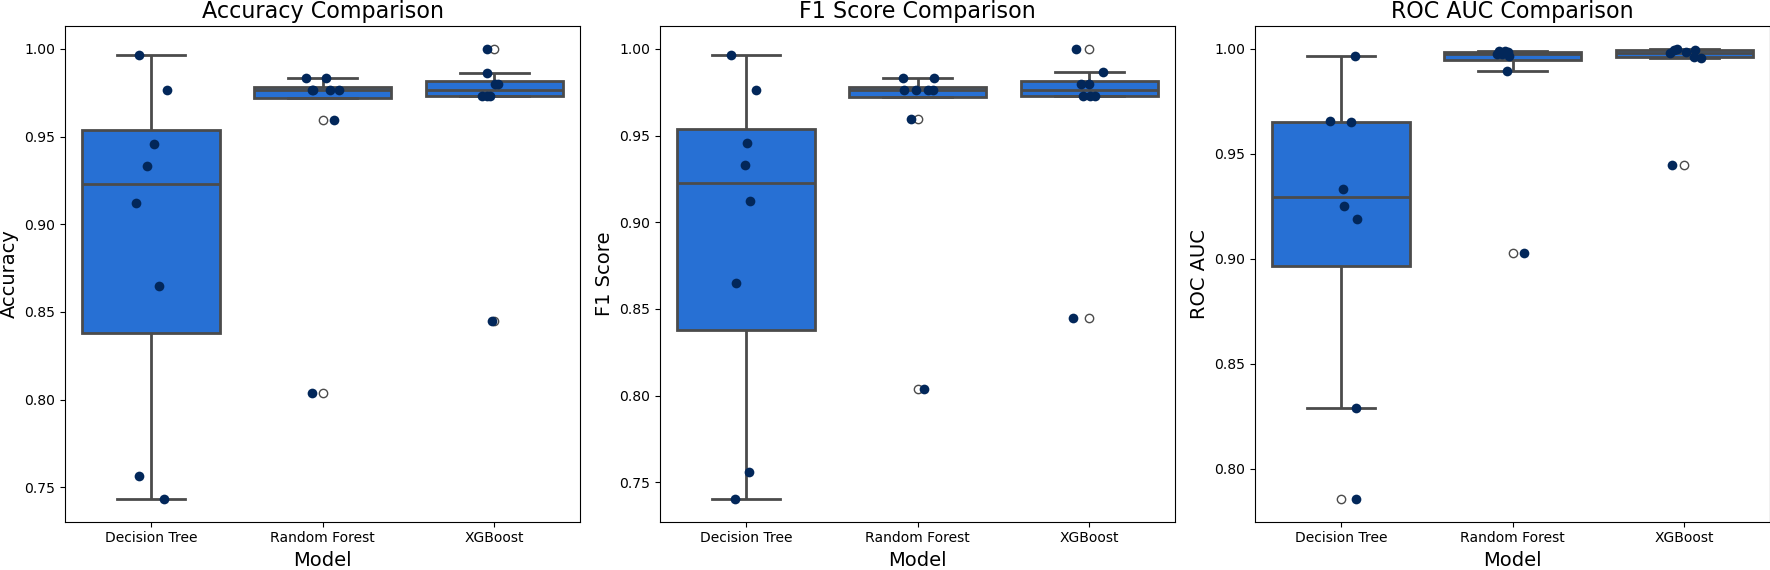
\includegraphics[width=460px]{ModelOptimization/box_plots_metrics.png}%
\caption{Boxplots of accuracy, f1, roc\_auc}%
\end{figure}

%
\subsection{Barplots of maximum values of metrics achievied by model}%
\label{subsec:Barplotsofmaximumvaluesofmetricsachieviedbymodel}%


\begin{figure}[h!]%
\centering%
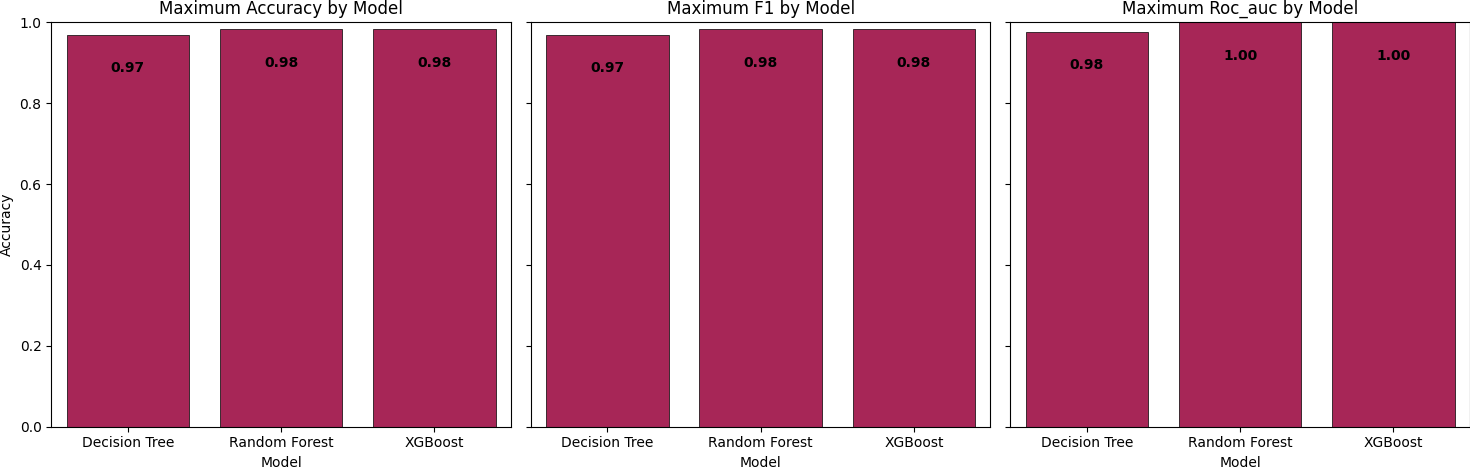
\includegraphics[width=460px]{ModelOptimization/barplots_max_metric.png}%
\caption{Barplots of maximum values of metrics achievied by model}%
\end{figure}

%
\end{document}